\begin{frame}[standout]
	\Huge \textsc{Outlook}
\end{frame}

\begin{frame}{Plan-Properties: Input}
	\centering
	\begin{tikzpicture}
		\node[draw, minimum width=3.5cm, minimum height=2.5cm] (framework) at (0,0) {\Large \textbf{Framework}};

		\visible<2->{
			\node[] (task) at (-3.8,1.3) {\Large \textbf{Problem}};
			\node[] (task2) at (-4.5,2.3) {
\includegraphics[scale=0.05]{images/rover1.png}};
			\node[] (task3) at (-3.1,2.3) {
\includegraphics[scale=0.05]{images/rover2.png}};
			\node[] (task4) at (-4.5,3.3) {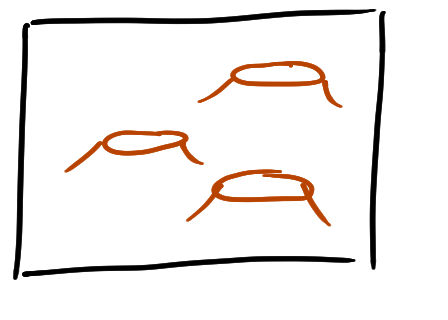
\includegraphics[scale=0.05]{images/image1.png}};
			\node[] (task5) at (-3.85,3.3) {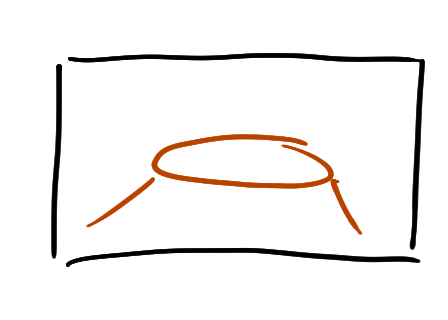
\includegraphics[scale=0.05]{images/image2.png}};
			\node[] (task6) at (-3.1,3.3) {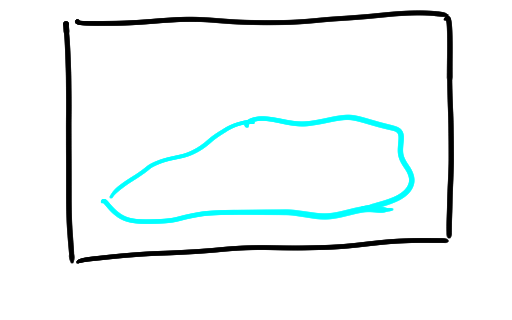
\includegraphics[scale=0.05]{images/image3.png}};
		}

		\visible<5->{
			\node[] (props) at (-3.8,-1.1) {\Large \textbf{Properties}};
			\node[draw, inner sep=1pt] (props1) at (-4.6,-2.5) {
				\resizebox{!}{1.2cm}{%
					\dontuseconnection{1}{1}{2}
				}
			};
			\node[draw, inner sep=1pt] (props2) at (-2.8,-2.5) {
				\resizebox{!}{1.2cm}{%
					\specificrover{1}{1}
				}
			};
		}
		\visible<6->{
			\node[] (no) at (-3.8,-1.8) {
\includegraphics[scale=0.3]{images/no.png}};
		}

		\visible<3->{
			\node[] (plan) at (3.8,1.3) {\Large \textbf{Plan}};
			\node[draw, align=left, fill=white] (plan2) at (4,3.0) {
					\scriptsize
					$drive(R_1,L_1,L2)$\\[-0.2cm]
					\scriptsize
					$takeImage_1(R_1)$\\[-0.2cm]
					\scriptsize
					$drive(R_2,L_4,L_5)$\\[-0.2cm]
					\scriptsize
					$takeImage_3(R_2)$\\[-0.2cm]
					\scriptsize
					$drive(R_2,L_5,L_6)$\\[-0.2cm]
					\scriptsize
					$\cdots$
			};
		}

		\visible<4->{
			\node[] (exp) at (3.8,-1.3) {\Large \textbf{Explanation}};
			\node[] (exp2) at (3.8,-2.5) {
				\resizebox{!}{1cm}{%
				\begin{tikzpicture}
					\node[draw] (p1) at (5,0) {
						\specificrover{1}{1}
					};

					\node[draw] (p4) at (0,0) {
						\dontuseconnection{1}{1}{2}
					};
					\node[] (not) at (5,0) {
\includegraphics[scale=0.3]{images/no.png}};

					\draw[thick, ->] (p4) to (p1);
				\end{tikzpicture}
				}
			};
		}

		\draw[->, line width=2pt] (-4,0) to (-2.5,0);
		\draw[->, line width=2pt] (2.5,0) to (4,0);

	\end{tikzpicture}
\end{frame}

\begin{frame}{Plan-Properties: Languages}
\centering
\begin{tikzpicture}
	\node[] (p1) at (-0.5,-3.5) {\samerover{1}{2}};
	\node[draw,inner sep=2pt] (p2) at (3,-3.5) {\orderprop{1}{2}};
	\node[draw,inner sep=2pt] (p3) at (6.5,-3.5) {\energylimit{1}};
	\node[] (p4) at (-0.5,0) {\specificrover{1}{2}};
	\node[] (p5) at (3,0) {\useconnection{1}{x}{y}};
	\node[] (p6) at (6.5,0) {\dontuseconnection{1}{x}{y}};
\end{tikzpicture}
\end{frame}

\begin{frame}{Iterative Planning}
	\centering
	%\begin{tikzpicture}
	%	\visible<2->{\node[draw, fill=blue!30] at (5.8,0) {Here is your $plan$.};}
	%	\visible<3->{\node[draw, fill=mLightGreen!30] at (-0.1,-1.2) {Why don't you avoid connection X ?};}
	%	\visible<4->{\node[draw, fill=blue!30, align=left] at (4.1,-2.4) {Because you would not be able to take\\ all image using a single rover.};}
	%	\visible<5->{\node[draw, fill=mLightGreen!30] at (0,-3.6) {I don't care about using more rovers.};}
	%	\visible<6->{\node[draw, fill=blue!30, align=left] at (4.6,-4.8) {Here is a new $plan'$ using two\\ rovers but avoiding connection X.};}
	%\end{tikzpicture}
	\begin{tikzpicture}
		\visible<1>{\node[] (i1) at (0,0) {
\includegraphics[scale=0.30]{images/iter/iter1.png}};}
		\visible<2>{\node[] (i2) at (0,0) {
\includegraphics[scale=0.30]{images/iter/iter2.png}};}
		\visible<3>{\node[] (i3) at (0,0) {
\includegraphics[scale=0.30]{images/iter/iter3.png}};}
		\visible<4>{\node[] (i4) at (0,0) {
\includegraphics[scale=0.30]{images/iter/iter4.png}};}
		\visible<4-5>{\node[] (i4) at (2.8,2.3) {
			\resizebox{!}{1.5cm}{%
			\begin{tikzpicture}
				\node[draw] (p1) at (5,0) {
					\specificrover{1}{1}
				};

				\node[draw] (p4) at (0,0) {
					\dontuseconnection{1}{1}{2}
				};
				\node[] (not) at (5,0) {
\includegraphics[scale=0.3]{images/no.png}};

				\draw[thick, ->] (p4) to (p1);
			\end{tikzpicture}
			}
		};}
		\visible<5>{\node[] (i5) at (0,0) {
\includegraphics[scale=0.30]{images/iter/iter5.png}};}
		\visible<6>{\node[] (i6) at (0,0) {
\includegraphics[scale=0.30]{images/iter/iter6.png}};}
	\end{tikzpicture}\\

\end{frame}


\begin{frame}{Why?}
	\centering
	\begin{tikzpicture}
		\node[] (p) at (3,1) {
			\resizebox{!}{2cm}{%
			\begin{tikzpicture}
				\node[draw] (p1) at (5,0) {
					\specificrover{1}{1}
				};

				\node[draw] (p4) at (0,0) {
					\dontuseconnection{1}{1}{2}
				};
				\node[] (not) at (5,0.9) {
\includegraphics[scale=0.1]{images/no.png}};

				\draw[thick, ->] (p4) to (p1);
				\visible<5->{
					\node[] (no) at (2.5,0) {
\includegraphics[scale=0.1]{images/no.png}};
				}
			\end{tikzpicture}
			}
		};
		
		\node[] (ai_exp) at (3,-2) {
\includegraphics[scale=0.2]{images/ai_exp.png}};

		\visible<2>{
			\node[] (child_why) at (-3,-1.0) {
\includegraphics[scale=0.22]{images/warum_darum.png}};
		}

		\visible<3>{
			\node[draw] (pa) at (-3,-1.5) {
				\energylimitloc{1}
			};
		}
		\visible<4->{
		\node[] (pa) at (-3,-1.5) {
			\begin{tikzpicture}
				\node[] (task1) at (-4.5,4.0) {\Large Planning Task};
				\node[] (task2) at (-4.9,1.8) {
\includegraphics[scale=0.07]{images/rover1.png}};
				\node[] (task3) at (-2.8,1.8) {
\includegraphics[scale=0.07]{images/rover2.png}};
				\node[] (task4) at (-4.7,3.3) {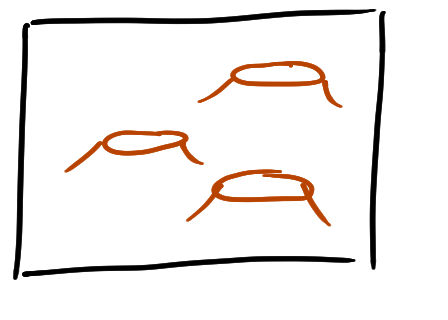
\includegraphics[scale=0.07]{images/image1.png}};
				\node[] (task5) at (-3.85,3.3) {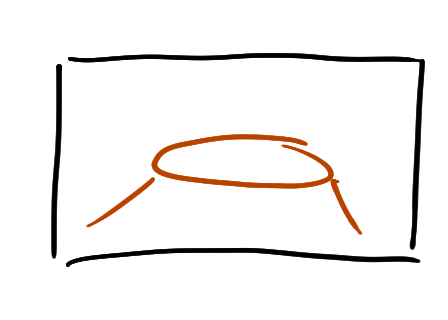
\includegraphics[scale=0.07]{images/image2.png}};
				\node[] (task6) at (-2.8,3.3) {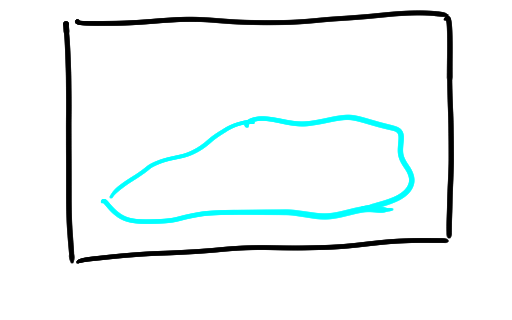
\includegraphics[scale=0.07]{images/image3.png}};
				\node[] (task7) at (-3.8,0.7) {
\includegraphics[scale=0.1]{images/battarie.png}};
				\visible<5->{
					\node[] (task7) at (-3.8,0.7) {
\includegraphics[scale=0.1]{images/no.png}};
				}
			\end{tikzpicture}
		};
		}
	\end{tikzpicture}\\

\end{frame}

\begin{frame}[plain]
	\centering
	\begin{tikzpicture}
		\node[draw, minimum width=3.5cm, minimum height=2.5cm] (framework) at (0,0) {\Large \textbf{Framework}};

		\node[] (task) at (-3.8,1.3) {\Large \textbf{Problem}};
		\node[] (task2) at (-4.5,2.3) {
\includegraphics[scale=0.05]{images/rover1.png}};
		\node[] (task3) at (-3.1,2.3) {
\includegraphics[scale=0.05]{images/rover2.png}};
		\node[] (task4) at (-4.5,3.3) {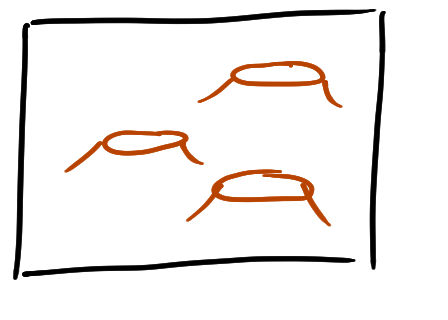
\includegraphics[scale=0.05]{images/image1.png}};
		\node[] (task5) at (-3.85,3.3) {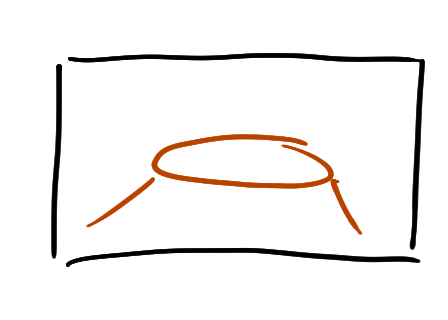
\includegraphics[scale=0.05]{images/image2.png}};
		\node[] (task6) at (-3.1,3.3) {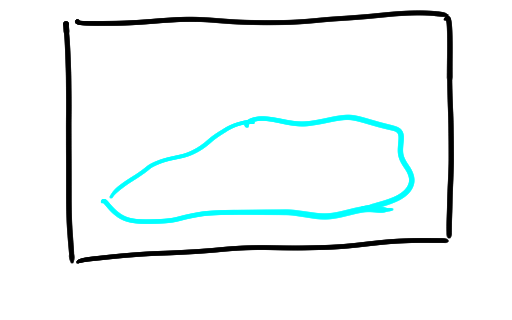
\includegraphics[scale=0.05]{images/image3.png}};

		\node[] (props) at (-3.8,-1.1) {\Large \textbf{Properties}};
		\node[draw, inner sep=1pt] (props1) at (-4.6,-2.5) {
			\resizebox{!}{1.2cm}{%
				\dontuseconnection{1}{1}{2}
			}
		};
		\node[draw, inner sep=1pt] (props2) at (-2.8,-2.5) {
			\resizebox{!}{1.2cm}{%
				\specificrover{1}{1}
			}
		};

		%\node[] (no) at (-3.8,-1.8) {
\includegraphics[scale=0.3]{images/no.png}};

		\node[] (plan) at (3.8,1.3) {\Large \textbf{Plan}};
		\node[draw, align=left, fill=white] (plan2) at (4,3.0) {
				\scriptsize
				$drive(R_1,L_1,L2)$\\[-0.2cm]
				\scriptsize
				$takeImage_1(R_1)$\\[-0.2cm]
				\scriptsize
				$drive(R_2,L_4,L_5)$\\[-0.2cm]
				\scriptsize
				$takeImage_3(R_2)$\\[-0.2cm]
				\scriptsize
				$drive(R_2,L_5,L_6)$\\[-0.2cm]
				\scriptsize
				$\cdots$
		};

		\node[] (exp) at (3.8,-1.3) {\Large \textbf{Explanation}};
		\node[] (exp2) at (3.8,-2.5) {
			\resizebox{!}{1cm}{%
			\begin{tikzpicture}
				\node[draw] (p1) at (5,0) {
					\specificrover{1}{1}
				};

				\node[draw] (p4) at (0,0) {
					\dontuseconnection{1}{1}{2}
				};
				\node[] (not) at (5,0) {
\includegraphics[scale=0.3]{images/no.png}};

				\draw[thick, ->] (p4) to (p1);
			\end{tikzpicture}
			}
		};

		\draw[->, line width=2pt] (-4,0) to (-2.5,0);
		\draw[->, line width=2pt] (2.5,0) to (4,0);

	\end{tikzpicture}

\end{frame}



